\documentclass[a4paper,10pt]{article}
\usepackage[utf8]{inputenc}
\usepackage[francais]{babel}

\usepackage{amsmath}
\usepackage{amsfonts}
\usepackage{amssymb}
\usepackage{amsthm}
\usepackage{xfrac}
\usepackage{graphicx}

\usepackage[T1]{fontenc}
\usepackage{type1cm}
\usepackage{lmodern}

\newtheorem{theorem}{Théorème}

\title{Informatique Scientifique par la Pratique\\Rapport du cours}
\author{Raphaël BERTHIER, Alban PIERRE et Luca WEHRSTEDT}

\begin{document}
\maketitle

\section{Swarm autohealing}

Au tout début nous étions intéressés par le problème de swarm autohealing, présenté au premier cours par Remi Geraud. Il s'agissait de modéliser le comportement d'un ensemble d'agents dispersés en espace qui, en conditions normales, produisent du profit pour la communauté. Cependant, un agent peut être compromis et commence à coûter. En ce cas ses agents voisins organisent un vote pour décider de tuer l'agent compromis ou de le réparer, avec des coûts liées à chaque option.

Le défi principal de ce problème était que c’était à nous de concevoir et proposer une formalisation appropriée. Nous avons donc commencé avec le cas le plus simple, où les agents ont information complète sur l’état de tout le système, sur le profit et le coût dans les différents régions de l'espace, sur le mouvement futur des autres agents. Nous avons étudié les cas d'un espace fini et d'un espace continu. En fait, la décision optimale des agents voisins pendant le vote était facile à déterminer : il fallait simplement estimer le gain futur de l'agent et le comparer avec le coût du sauvetage. Le calcul consiste en la résolution d'un système linéaire dans le cas discret et d'une équation intégrale dans le cas continu.

Généraliser le problème à une modélisation où les agents ne disposent que d'une information partielle s'est révélé beaucoup plus ardu. Cependant, cette situation est au centre de l'intérêt du problème de swarm autohealing. En effet, les agents n'ont accès qu'à une information locale, ce qui fait qu'ils ne connaissent pas l'ensemble du système - ni son évolution à fortiori. Par ailleurs, c'est pour cela que les prises de décision des différents agents diffèrent : ceci constitue tout l'intérêt de la phase de vote des agents. Il était donc essentiel que notre modélisation du problème prenne en compte la localité de l'information.

Cependant, nous n'avons abouti à aucun résultat d'intérêt avec ce modèle. Il nous a semblé que le mieux que nous puissions faire était de procéder comme dans le cas à information totale, mais en acceptant le manque d'information qui engendre une part d'aléatoire dans le problème. Pour être précis, un agent doit estimer les informations qui lui manquent, pour ensuite prévoir si il est avantageux de sauver un agent corrompu ou non.

Remarquons cependant que puisque ce mode de prise de décision est dangereux, puisque une petite erreur dans l'estimation des paramètres inconnus peut avoir de grandes conséquences : tuer plutôt que sauver. Pour y remédier, on peut rendre les décisions des agents aléatoires : tuer avec probabilité $p$, sauver avec probabilité $1-p$, où $p$ dépend des paramètres (estimés) du système. Cela permet d'éviter un ``effet seuil'' où de petites variations des paramètres auraient de grandes conséquences.

Mais, n'étant pas plus inspirés par ce modèle, nous avons donc décidé d'abandonner cette direction et de nous dédier à un problème différente.

\section{Modèle de Krause pour la dynamique d'opinion}

Dans le modèle de Krause on étudie des agents (normalement un nombre fini, mais ils existent des généralisations à un nombre infini, dénombrable ou continu) qui sont caractérisés par leur opinion, qui est une valeur dans un certain espace métrique (normalement un intervalle borné de $\mathbb{R}$). Le système évolue à temps discret. A chaque étape tous les agents se déplacent en même temps vers la moyenne des positions des agents qui leur sont proches, c'est-à-dire qui ont une distance inférieure à 1. Formellement, dans le cas le plus simple d'un nombre fini d'opinions réelles, on pourrait dire que
\begin{equation}
x_i^{(t+1)} = \frac{1}{|N_d^{(t)}(i)|} \sum_{j \in N_d^{(t)}(i)} x_j^{(t)}
\end{equation}
où $N_d^{(t)}(i) = \{j \text{ t.q. } |x_j^{(t)} - x_i^{(t)}| < d\}$.
Cette équation vise à modéliser le phénomène d'influence suivant : un agent est influencé par les opinions des autres agents, sous réserve qu'ils aient une opinion pas trop différente de la sienne. Autrement dit, nous sommes hermétiques aux gens qui pensent très différemment de nous. En revanche, lorsque quelqu'un pense légèrement différemment de nous, nous modifions notre opinion en prenant en compte la sienne.

\subsection{Aperçu de notre travail théorique}

Pour nous donner des suggestions, le professeur nous a envoyé une présentation qu'il avait fait pour synthétiser et commenter l'article ``On Krause’s multi-agent consensus model with state-dependent connectivity'' de Vincent D. Blondel, Julien M. Hendrickx et John N. Tsitsiklis. Le thème nous intéressait et nous avons donc décidé de lire l'article original en entier pour mieux comprendre le modèle, les problématiques et les approches proposées.

Un premier aspect que nous avons étudié a été la distribution des instants auxquels deux groupes d'agents s'unifient. Pour cela nous avons écrit un simulateur spécialisé et optimisé pour exécuter un grand nombre de fois des simulations à partir d'une situation aléatoire et obtenir des données statistiques. En représentant ces graphiques nous n'avons trouvé aucun comportement facilement descriptible et donc nous avons abandonné cette piste.

Cependant, nous avons trouvé dans l'article de nouveaux problèmes ouverts, qui viennent compléter ceux que le professeur a écrit dans sa présentation. En particulier dans une section de commentaire les auteurs disent qu'un résultat qu'il venaient de prouver (la convergence au clusters séparés d'au moins $d$) n'est pas vrai dans n'importe quel espace. Ils donnaient comme contre-exemple le cas d'agents placés sur le cercle et ils disaient que dans ce cas, même la simple convergence n’était pas prouvée. Ainsi nous avons décidé de travailler sur ce problème.

Au tout début nous avons écrit un simulateur en Python, pour nous aider à mieux comprendre les différentes situations qui peuvent se présenter. Nous avons distingué deux modes de convergence :

\begin{itemize}
\item Si lors qu'un des étapes de la convergence, il se forme un ``trou'' de taille au moins $d$ entre deux agents successifs, alors ce trou ne peut plus se réduire. Puisque les deux agents successifs ne sont plus en influence, tout se passe alors comme si on était ramené au cas réel, en ``coupant'' le cercle au niveau du trou. Le phénomène est alors connu, et on a convergence vers des clusters séparés par une distance au moins $d$. On donne dans les figurs \ref{randombefore}, \ref{random2} et \ref{random5} une illustration de ce phénomène, sur le cercle de rayon $1$, avec $d = 1$.

\begin{figure}
\center
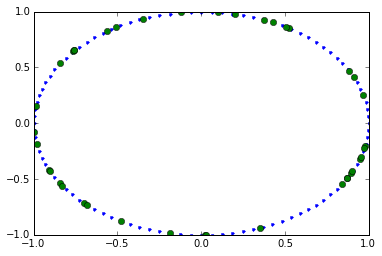
\includegraphics[scale=0.5]{randombefore.png}
\caption{Distribution initiale. Tous les agents sont à distance inférieure ou égale à $d$.}
\label{randombefore}
\center
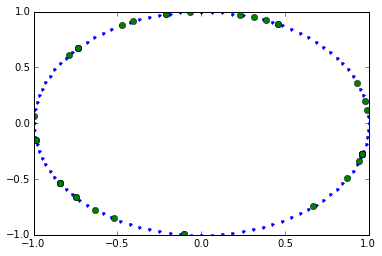
\includegraphics[scale=0.5]{random2.png}
\caption{Après deux itérations. Des trous commencent à se former à cause des différences de concentration en agents le long du cercle.}
\label{random2}
\center
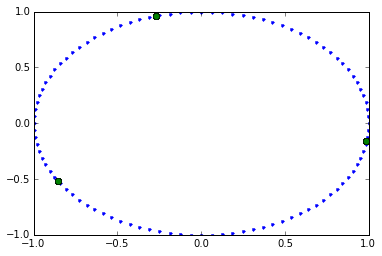
\includegraphics[scale=0.5]{random5.png}
\caption{Après cinq itérations. Trois clusters se sont formés, à des distances plus grandes que $d$.}
\label{random5}
\end{figure}

\item Cependant, il est possible que les couples d'agents successifs ne se séparent jamais d'une distance de plus de $d$. Par exemple, prenons $n$ suffisamment grand, et plaçons des $n$ agents sur les racines $n$-ièmes de l'unité. Chaque agents sera influencé par ses voisins, mais les influences se compensent exactement, de sorte que la distribution est stable. Nous avons ici ce que nous appelons une convergence non standard, c'est-à-dire que des agents restent sous influence mutuelle, bien qu'ils ne convergent pas vers la même position.
En modifiant légèrement et aléatoirement la position initiale des agents par rapport à cette distribution, nous avons constaté numériquement que cette distribution est stable. Nous montrons une de ces simulations numériques dans les figures \ref{racinesbefore} et \ref{racines1000}, ainsi qu'une preuve théorique de ce résultat dans le théorème \ref{convergence-non-standard}.

\begin{figure}
\center
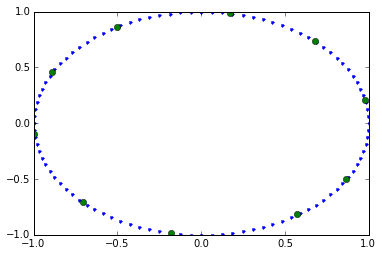
\includegraphics[scale=0.5]{racinesbefore.png}
\caption{Une distribution proche des racines 10-ième de l'unité, sur les cercle trigonométrique, avec $d=1$.}
\label{racinesbefore}
\center
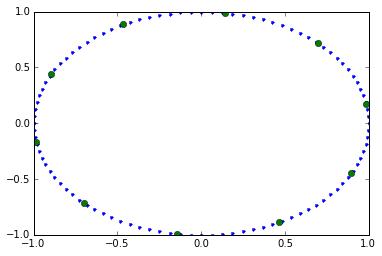
\includegraphics[scale=0.5]{racines1000.png}
\caption{Le même système, après 1000 itérations.}
\label{racines1000}
\end{figure}

\end{itemize}

Nous avons de plus constaté qu'en choisissant les positions initiales des agents indépendamment et uniformément sur le cercle, on obtenait nettement plus fréquemment une convergence standard.

Pour continuer à nous familiariser avec le modèle, cette fois ci d'un point de vue théorique, nous avons essayé de démontrer un résultat ``préliminaire'' : l'ensemble des situations initiales qui conduisent à une convergence non standard n'est pas de mesure nulle (en supposant la distribution de probabilité obtenue en tirant uniformément et indépendamment chaque agent). Cela nous a confirmé ce que nous avions vu expérimentalement : les situations que nous voulions analyser ne sont pas négligeables.

\begin{theorem}
\label{convergence-non-standard}
Considérons $n$ agents placés sur le cercle de rayon 1 et soit $d$ la distance d'influence. La position de l'agent $i$ est $x_i = r_i + b_i$ où $r_i = \frac{i}{n} 2 \pi$ et $b_i \in (-\epsilon, +\epsilon)$. Alors la convergence sera non standard pour un $\epsilon$ suffisamment petit.
\end{theorem}

Nous avons supposé que le bruit n'arrive pas à changer les relations d'influence entre les agents. On peut formaliser cela comme une contrainte sur $\epsilon$ : pour aucun $k \ge 1$ on peut avoir $\frac{k}{n} 2 \pi - 2\epsilon < d < \frac{k}{n} 2 \pi + 2\epsilon$.

Après des essais numériques nous nous sommes convaincus que une situation de ce type converge vers une distribution équidistante, où l'agent $i$ est à la position $r_i + \bar b$, avec $\bar b = \frac{1}{n} \sum_{j=1}^n b_j$. Nous avons trouvé une preuve de ce résultat on utilisant les chaînes de Markov :

\begin{proof}
A chaque étape, chaque agent est influencé par autant d'agents à gauche que à droite. Soit $k$ ce nombre. Donc à la deuxième étape
\begin{equation*}
\begin{split}
x'_i &= \frac{1}{2k+1} \left( \sum_{j=1}^k x_{i-j} + x_i + \sum_{j=1}^k x_{i+j} \right) \\
     &= \frac{1}{2k+1} \left( \sum_{j=1}^k (r_{i-j} + b_{i-j}) + r_i + b_i + \sum_{j=1}^k (r_{i+j} + b_{i+j}) \right) \\
     &= \frac{1}{2k+1} \left( \sum_{j=1}^k (r_i - \frac{j}{n}2 \pi + b_{i-j}) + r_i + b_i + \sum_{j=1}^k (r_i + \frac{j}{n}2 \pi + b_{i+j}) \right) \\
     &= \frac{1}{2k+1} \left( \sum_{j=1}^k (r_i + b_{i-j}) + r_i + b_i + \sum_{j=1}^k (r_i + b_{i+j}) \right) \\
     &= r_i + \frac{1}{2k+1} \left( \sum_{j=1}^k b_{i-j} + b_i + \sum_{j=1}^k b_{i+j} \right) \\
\end{split}
\end{equation*}

On voit donc que le nouveau bruit de l'agent $i$ est la moyenne des bruits des agents voisins. En itérant le raisonnement on obtient qu'à tout moment $t$ le bruit d'un agent $i$ est une combinaison linéaire à coefficients $\alpha_{i,j}^{(t)}$ des bruits initiaux $b_j$ de tous les agents. On peut donc fixer un $j$ et voir comment évoluent les $\alpha_{i,j}^{(t)}$. Au début ils sont tous nuls sauf celui de l'agent $j$ lui-même, $\alpha_{j,j}^{(0)}$, qui vaut 1. A l’étape suivante on voit que les $2k+1$ voisins de $j$ (y compris $j$) ont le coefficient $\alpha_{i,j}^{(1)}=\frac{1}{2k+1}$ ; les autres ont ce coefficient à 0. La somme reste donc 1. En fait c'est une propriété qui vaut pour toute étape, car chacun des $2k+1$ voisins d'un agent a lui aussi $2k+1$ voisins. Cela nous permet de considérer ces coefficients comme une distribution de probabilité et ensuite de voir l’évolution du système comme une chaîne de Markov. Cette chaîne est irréductible, apériodique et, ayant un nombre fini d'états, récurrente positive. Elle converge donc vers une distribution stationnaire, qui est la distribution uniforme. Le bruit initial de l'agent $j$ se disperse donc en proportions égales entre tous les agents. A la limite tous les agents auront le même bruit qui sera la moyenne des bruits initiaux.
\end{proof}

Par la suite nous avons abordé le théorème principal : il y a toujours convergence, soit standard soit non standard. Le théorème précédent en est un cas particulier mais nous ne pouvions pas utiliser les mêmes techniques sans modification parce que plusieurs hypothèses n’étaient plus valides. En particulier la somme des coefficients de la contribution de l'agent $j$ dans la position des autres agents ne reste pas 1. Aussi, la relation d'influence peut changer à chaque étape, vu que des agents peuvent s'approcher ou s’éloigner l'un de l'autre. Autrement dit, la chaîne de Markov n'est pas homogène.

Nous avons quand même essayé de nous ramener à la situation précédente en supposant qu'à partir d'un certain rang, la relation d'influence arrête de changer. Cela implique aussi que la matrice de transition ne change plus, et donc nous pouvons l'analyser. C'est une matrice stochastique, parce que la somme des poids des arêtes qui entrent dans un agent vaut 1 (les $n$ arêtes ont toutes le même poids, qui est $\frac{1}{n}$). Les arêtes sortantes, au contraire, n'ont pas forcément somme 1. Donc, même si cette matrice est stochastique, on ne peut pas l'utiliser pour modéliser une chaîne de Markov parce que on l'utiliserait ``dans le mauvais sens'' : elle est stochastique gauche (par colonnes) mais on la multiplierait par un vecteur ligne. En tout cas, en étant stochastique, nous sachons que sa puissance $n$-ième a une limite, et donc de cela nous déduisons que les positions des agents convergent (le vecteur qui les décrit est obtenu par la multiplication de cette matrice et du vecteur des positions à l'instant auquel la relation d'influence se stabilise).

Il nous ne restait donc que à prouver que la relation se stabilise après un certain temps fini. Nous avions commencé à chercher une mesure qui décroissait, ou un argument pour prouver que dès qu'on revenait de nouveau sur une configuration déjà visitée on commençait à boucler, etc. A un certain point nous sommes tombés sur une prépublication de ArXiV, d'un article qui paraissait démontrer exactement le résultat qui nous avions envisagé : ``The Hegselmann-Krause Dynamics on the Circle Converge'', écrit par Peter Hegarty, Anders Martinsson et Edvin Wedin. En le lisant nous avons en fait retrouvé notre schéma de preuve, exactement l’idée de utiliser la stabilité de la relation d'influence comme étape intermédiaire. Ils avaient prouvé la seconde partie en adaptant l’idée d'``énergie'' déjà introduite dans un autre papier, pour laquelle il fallait considérer une version orientée de la relation d'influence. D'après eux, l'idée est ``bien connue''. Nous pensons donc que une faute que nous avons commis dans le déroulement de notre projet est de ne pas avoir donné suffisamment de temps à la lecture de la littérature existante.

\subsection{Essais pratiques}

Nous avons fait un programme pour calculer puis afficher les opinions au cours du temps, ces opinion étaient un entier entre 0 et 1. Nous avons testé selon plusieurs modèles : (on note $d$ la distance d'opinion entre la personne influencée et la personne influente)
\begin{enumerate}
\item Créneau : une personne écoute les personnes d'opinion qui diffère de moins de $D \in \mathbb{R}$, toutes avec le même coeff, et pas les autres. Autrement dit la fonction qui donne le coefficient de prise en compte d'opinion en fonction de la distance d est un créneau de largeur 2D.

\item Inverse : la fonction $\operatorname{coeff}(d)$ est $\sfrac{1}{(1+d)}$.

\item Inverse au carré : la fonction $\operatorname{coeff}(d)$ est $\sfrac{1}{(1+d^2)}$.

\item Inverse au carré bis : la fonction $\operatorname{coeff}(d)$ est $\min(\sfrac{1}{d^2}, D)$ et $D$ en $d=0$.

\item Gaussien : la fonction $\operatorname{coeff}(d)$ est une gaussienne de variance $D \in \mathbb{R}$.
\end{enumerate}

Nous avons bien sûr fait varié $D$ et regardé les différences obtenues. Assez logiquement, plus $D$ est grand moins il y a d'opinions finales.

Certaines de ces fonctions faisaient converger très rapidement (ex : créneau vers $t \sim 5$) alors que d'autres beaucoup plus lentement (inverse au carre vers $t \sim 30000$). C'est pourquoi nous avons essayé plusieurs fonctions d'affichage :
\begin{enumerate}
\item affichage linéaire : la valeurs de l'opinion en ordonnée et le temps en abscisse, le temps ayant pour échelle 1pixel/1unité de temps jusqu'à 100pixels/1unité de temps.

\item affichage linéaire cyclique : comme l'affichage linéaire, sauf qu'une fois arrivé au bout de la fenetre on efface tout puis on affiche la suite, etc.

\item affichage logarithmique : l'abscisse est $\log(t)$, c'est à dire qu'une valeur au temps $t$ est affiché sur le pixel d'abscisse $\log(t)$.
\end{enumerate}

Face à la rapidité de la convergence de certains modèles, nous avons implémenté l'inertie : plus cette inertie est importante, moins l'opinion de la personne change. C'est à dire que la personne prend en compte son opinion avec un coeff proportionnel à l'inertie. Cela permet de ralentir la convergence et d'obtenir des courbes plus jolies.
Nous avons aussi essayé une version où l'inertie change selon les personnes.

Nous avons ensuite ajouté du bruit, ie une personne a une opinion qui monte ou descend aléatoirement (en plus du changement d'opinion dû aux autres personnes) à chaque unité de temps. Nous avons mis un bruit à peu près gaussien. Ainsi nous obtenons selon les modèles une ou plusieures opinions principales qui bougent légèrement, qui sont larges avec un gros bruit et fines avec un petit bruit. Celles-ci se rejoignent parfois. De plus avec un bruit suffisament fort certaines personnes sortent des idées principales. Avec un bruit très fort on observe plus rien; et entre les deux on observe des idées principales qui bougent beaucoup, se rejoignent, se divisent, des trous d'opinions qui se créent puis disparaisent : c'est assez proche de la réalité.
Nous avons rencontré un problème dû à la fonction \texttt{rand()} en c : en utilisant beaucoup cette fonction, nous obtenous de l'aléatoire qui se répète, et du coup des opinions de personnes qui montent et descendent de la même manière.

Nous avons ensuite essayé une version où les valeurs des opinions sont sur un cercle, cela n'a pas changé grand chose.

Enfin nous avons rajouté quelques petites choses, comme le choix des couleurs pour afficher les opinions, le choix des opinions au départ (aléatoire, uniformément réparti, tous au centre, ...) ou encore l'essai d'une mesure de 'chaos' qui est la somme pour toutes les personnes de la somme des coefficient d'influence.


\end{document}